\section{Mô hình và phương pháp giải quyết bài toán}

Phần này trình bày phương pháp và quy trình giải quyết bài toán phân loại đánh giá sản phẩm thời trang nữ (\textit{Women's E-Commerce Clothing Reviews}). Dữ liệu được đưa qua các giai đoạn: biểu diễn văn bản, lựa chọn đặc trưng, huấn luyện các mô hình học máy gồm Support Vector Machine (SVM), Logistic Regression, Multinomial Naive Bayes và XGBoost, cùng các kỹ thuật nâng cao gồm tối ưu siêu tham số, học kết hợp (Ensemble Learning) và tích hợp siêu dữ liệu (Metadata).

\subsection{Biểu diễn dữ liệu văn bản (Text Representation)}
Trước khi đưa dữ liệu vào các mô hình học máy, văn bản đánh giá được chuyển đổi từ dạng chuỗi ký tự ban đầu sang vector đặc trưng số thông qua quá trình Tokenization. Các đánh giá có \texttt{Review Text} hoặc \texttt{Title} khuyết thiếu được xử lý điền chuỗi rỗng và ghép nối thành một trường văn bản thống nhất.

\subsubsection{So sánh phương pháp Tokenization}
Nhóm tiến hành so sánh hai phương pháp mã hóa văn bản phổ biến bằng một mô hình chuẩn (\textit{LinearSVC}) trên tập dữ liệu:
\begin{itemize}
    \item \textbf{CountVectorizer}: Biểu diễn mỗi từ bằng tần số xuất hiện trong văn bản (Bag-of-Words), không xét thứ tự từ.
    \item \textbf{TfidfVectorizer}: Đếm số lần xuất hiện của từ trong văn bản và chuẩn hóa bằng nghịch đảo tần suất xuất hiện của từ đó trên toàn bộ tập dữ liệu (TF-IDF).
\end{itemize}

\begin{table}[H]
\centering
\begin{tabular}{|l|c|c|c|}
\hline
\textbf{Phương pháp Tokenize} & \textbf{Accuracy} & \textbf{F1-Score} & \textbf{Thời gian (giây)} \\ \hline
CountVectorizer & 0.8734 & 0.9238 & 4.05 \\ \hline
TfidfVectorizer & \textbf{0.8902} & \textbf{0.9348} & \textbf{1.40} \\ \hline
\end{tabular}
\caption{So sánh hiệu năng giữa CountVectorizer và TfidfVectorizer trên mô hình LinearSVC}
\label{tab:tokenizers_eval}
\end{table}

Kết quả thực nghiệm ở Bảng~\ref{tab:tokenizers_eval} cho thấy \texttt{TfidfVectorizer} vừa đạt hiệu năng vượt trội vừa có thời gian thực thi nhanh hơn rõ rệt (1.40 giây so với 4.05 giây), do đó \texttt{TfidfVectorizer} được lựa chọn làm phương pháp trích xuất đặc trưng chính cho toàn bộ quy trình.

\subsubsection{Cơ sở toán học của TF-IDF}
TF-IDF giảm trọng số của các từ xuất hiện phổ biến trong nhiều văn bản và tăng trọng số của các từ có tính phân biệt cao:
\begin{equation}
\text{tfidf}(t, d) = \text{tf}(t, d) \times \text{idf}(t), \qquad \text{idf}(t) = \ln\frac{1 + n}{1 + \text{df}(t)} + 1
\end{equation}
Trong đó, $n$ là tổng số văn bản trong tập dữ liệu và $\text{df}(t)$ là số văn bản có chứa từ $t$. Đây là công thức có làm trơn (smooth IDF) theo cài đặt của scikit-learn. Các vector đặc trưng sau đó được chuẩn hóa theo chuẩn $L_2$:
\begin{equation}
v_{\text{norm}} = \frac{v}{\|v\|_2} = \frac{v}{\sqrt{\sum_j v_j^2}}
\end{equation}
Ngoài ra, kỹ thuật \texttt{sublinear\_tf=True} được sử dụng nhằm thay thế tần suất từ $\text{tf}$ bằng $1 + \ln(\text{tf})$, giúp giảm thiểu ảnh hưởng áp đảo của các từ lặp lại quá nhiều lần. Các ngưỡng \texttt{min\_df} (loại bỏ từ hiếm) và \texttt{max\_features} (giới hạn từ vựng) được đưa vào kiểm thử để tránh làm bùng nổ số chiều. Để ngăn chặn hoàn toàn hiện tượng rò rỉ dữ liệu (\textit{data leakage}), bộ trích xuất đặc trưng được đặt bên trong cấu trúc \texttt{Pipeline}, đảm bảo từ vựng và trọng số IDF chỉ được học trên phần tập huấn luyện của từng fold trong quá trình kiểm định chéo.

\subsection{Lựa chọn đặc trưng (Feature Selection)}
Dữ liệu văn bản sau khi chuyển sang không gian n-gram thường tạo ra số chiều rất lớn chứa nhiều đặc trưng thưa và từ nhiễu. Kỹ thuật lựa chọn đặc trưng theo phương pháp lọc (\textit{Filter Method}) thông qua \texttt{SelectKBest} được áp dụng với hai hàm tính điểm thống kê:
\begin{itemize}
    \item \textbf{Chi-Square ($\chi^2$)}: Kiểm tra tính độc lập thống kê giữa sự xuất hiện của từ và nhãn phân loại:
    \begin{equation}
    \chi^2 = \sum \frac{(O - E)^2}{E}
    \end{equation}
    với $O$ là tần số quan sát thực tế và $E$ là tần số kỳ vọng theo giả thiết độc lập.
    \item \textbf{ANOVA F-Score}: Đánh giá tỷ số phương sai giữa các nhóm nhãn với phương sai nội bộ từng nhóm ($F = \frac{\text{MSB}}{\text{MSW}}$).
\end{itemize}

Nhóm tiến hành khảo sát số lượng đặc trưng giữ lại $k \in \{500, 1000, 2000, 3000\}$ trên mô hình LinearSVC:

\begin{table}[H]
\centering
\begin{tabular}{|c|c|c|}
\hline
\textbf{Số lượng đặc trưng $k$} & \textbf{ANOVA F-Score} & \textbf{Chi-Square ($\chi^2$)} \\ \hline
500  & 0.9378 & 0.9361 \\ \hline
1000 & 0.9393 & 0.9383 \\ \hline
2000 & 0.9380 & 0.9382 \\ \hline
3000 & 0.9366 & 0.9369 \\ \hline
\end{tabular}
\caption{F1-Score của các phương pháp lựa chọn đặc trưng theo số lượng đặc trưng $k$}
\label{tab:fs_eval}
\end{table}

\begin{figure}[H]
\centering
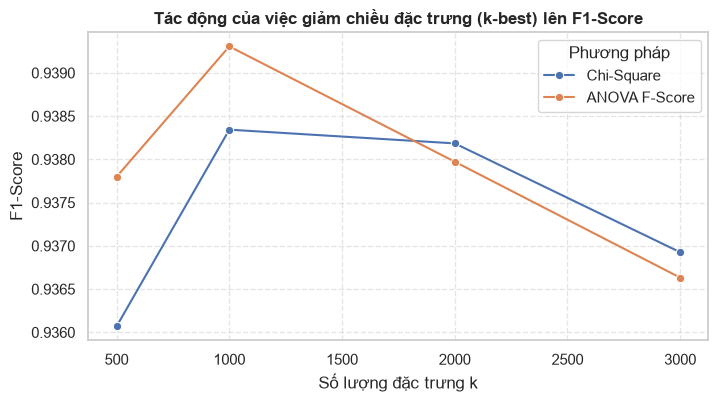
\includegraphics[width=0.7\textwidth]{figures/svm_cell17_0.png}
\caption{Tác động của việc giảm chiều đặc trưng ($k$-best) lên F1-Score}
\label{fig:fs_chart}
\end{figure}

Qua Bảng~\ref{tab:fs_eval} và Hình~\ref{fig:fs_chart}, việc rút gọn không gian đặc trưng về khoảng $k = 1000 \div 2000$ giúp duy trì và tối ưu F1-score so với việc giữ lại toàn bộ từ vựng, đồng thời làm giảm đáng kể chi phí tính toán trong các bước huấn luyện tiếp theo.

\subsection{Các mô hình học máy giải quyết bài toán}
Bốn thuật toán học máy được triển khai để giải quyết bài toán phân loại nhị phân (0: Không đề xuất, 1: Có đề xuất sản phẩm):

\subsubsection{Support Vector Machine (SVM)}
Mô hình Support Vector Machine tìm kiếm một siêu phẳng phân tách hai lớp sao cho khoảng cách (lề - margin) từ các điểm luyện tập gần nhất (các Support Vector) đến ranh giới quyết định là lớn nhất. Để giải quyết bài toán khi các lớp không thể phân tách tuyến tính trực tiếp trong không gian ban đầu, các hàm Kernel $K(x, x') = \langle \phi(x), \phi(x') \rangle$ được ứng dụng để ánh xạ các điểm dữ liệu vào không gian nhiều chiều hơn. Bốn dạng Kernel được khảo sát:
\begin{itemize}
    \item \textbf{Linear Kernel}: Tìm siêu phẳng trực tiếp trong không gian gốc:
    \begin{equation}
    K(x, x') = x^\top x'
    \end{equation}
    \item \textbf{Radial Basis Function (RBF) Kernel}: Ánh xạ dữ liệu vào không gian vô hạn chiều dựa trên khoảng cách Euclidean:
    \begin{equation}
    K(x, x') = \exp\left(-\gamma \|x - x'\|^2\right)
    \end{equation}
    \item \textbf{Polynomial Kernel}: Ánh xạ phi tuyến thông qua việc kết hợp các bậc lũy thừa:
    \begin{equation}
    K(x, x') = (\gamma x^\top x' + r)^d \quad (d=2)
    \end{equation}
    \item \textbf{Sigmoid Kernel}: Hoạt động tương tự hàm kích hoạt nơ-ron, phù hợp với dữ liệu nhị phân thưa:
    \begin{equation}
    K(x, x') = \tanh\left(\gamma x^\top x' + r\right)
    \end{equation}
\end{itemize}

\begin{table}[H]
\centering
\begin{tabular}{|l|c|c|c|}
\hline
\textbf{SVM Kernel} & \textbf{Accuracy} & \textbf{F1-Score} & \textbf{Thời gian huấn luyện (giây)} \\ \hline
SVC (Linear) & 0.8817 & 0.9307 & 6.21 \\ \hline
SVC (RBF) & 0.8721 & 0.9268 & 9.49 \\ \hline
SVC (Poly, deg=2) & 0.8550 & 0.9181 & 11.34 \\ \hline
SVC (Sigmoid) & \textbf{0.8819} & \textbf{0.9309} & \textbf{6.19} \\ \hline
\end{tabular}
\caption{So sánh hiệu năng các hàm Kernel của SVM trên tập dữ liệu thử nghiệm}
\label{tab:kernel_eval}
\end{table}

Kernel Sigmoid mang lại F1-score cao nhất (0.9309) cùng thời gian huấn luyện nhanh nhất (6.19 giây), tiếp theo là Linear Kernel. Cả hai được đưa vào không gian tìm kiếm siêu tham số chi tiết ở giai đoạn sau.

\subsubsection{Hồi quy Logistic (Logistic Regression)}
Logistic Regression ước lượng xác suất hậu nghiệm một quan sát thuộc lớp 1 thông qua hàm kích hoạt sigmoid:
\begin{equation}
P(y = 1 \mid x) = \sigma(w^\top x + b) = \frac{1}{1 + e^{-(w^\top x + b)}}
\end{equation}
Mô hình gán nhãn 1 khi $P(y = 1 \mid x) \ge 0.5$. Để kiểm soát nguy cơ quá khớp và xử lý bài toán mất cân bằng lớp (82.2\% lớp 1 và 17.8\% lớp 0), hàm mục tiêu sử dụng chuẩn hóa $L_2$ cùng trọng số mẫu $s_i$:
\begin{equation}
\min_{w, b} \frac{1}{2} \|w\|_2^2 + C \sum_i s_i \left[-y_i \ln p_i - (1 - y_i) \ln(1 - p_i)\right]
\end{equation}
Trong đó, $C$ là nghịch đảo của cường độ điều chuẩn. Tham số \texttt{class\_weight='balanced'} tự động gán trọng số $s_i$ nghịch với tần suất của các lớp nhằm bù đắp cho lớp thiểu số. Thuật toán tối ưu \texttt{lbfgs} được sử dụng nhằm hội tụ nhanh trên ma trận TF-IDF thưa.

\subsubsection{Multinomial Naive Bayes}
Multinomial Naive Bayes áp dụng định lý Bayes kết hợp giả định độc lập có điều kiện giữa các từ khi biết trước nhãn lớp:
\begin{equation}
P(c \mid d) \propto P(c) \prod_t P(t \mid c)^{x_t}
\end{equation}
Dạng tương đương trên thang đo logarit (log-posterior) là:
\begin{equation}
\hat{c} = \arg\max_c \left[ \ln P(c) + \sum_t x_t \ln P(t \mid c) \right]
\end{equation}
Xác suất có điều kiện của từ $t$ trong lớp $c$ được ước lượng bằng phương pháp làm trơn cộng Lidstone/Laplace:
\begin{equation}
\hat{\theta}_{ct} = \frac{N_{ct} + \alpha}{N_c + \alpha |V|}
\end{equation}
với $\alpha > 0$ là hệ số làm trơn giúp tránh xác suất bằng 0 cho các từ chưa xuất hiện, $N_{ct}$ là tổng trọng số TF-IDF của từ $t$ trong lớp $c$, và $|V|$ là kích thước từ vựng. Mô hình có chi phí tính toán rất thấp và hoạt động trực tiếp trên các giá trị TF-IDF không âm.

\subsubsection{XGBoost (Extreme Gradient Boosting)}
XGBoost là thuật toán gradient boosting xây dựng một tổ hợp cộng dồn tuần tự gồm các cây quyết định. Tại mỗi bước lặp $t$, một cây mới $f_t(x_i)$ được bổ sung để tối ưu hàm mục tiêu:
\begin{equation}
\hat{y}_i^{(t)} = \hat{y}_i^{(t-1)} + \eta f_t(x_i)
\end{equation}
với $\eta$ là tốc độ học (\textit{learning rate}). Hàm mục tiêu bao gồm hàm mất mát logistic kết hợp thành phần điều chuẩn kiểm soát độ phức tạp của cây:
\begin{equation}
\mathcal{L} = \sum_i \ell(y_i, \hat{y}_i) + \sum_k \Omega(f_k), \qquad \Omega(f) = \gamma T + \frac{1}{2} \lambda \|w\|^2
\end{equation}
trong đó $T$ là số lượng nút lá và $w$ là vector trọng số tại các lá. Bằng khai triển Taylor bậc hai của hàm mất mát, trọng số tối ưu tại lá $j$ được tính trực tiếp:
\begin{equation}
w_j^* = -\frac{G_j}{H_j + \lambda}
\end{equation}
với $G_j = \sum_{i \in I_j} g_i$ và $H_j = \sum_{i \in I_j} h_i$ lần lượt là tổng gradient bậc một và bậc hai của các mẫu thuộc lá $j$.

Để xử lý mất cân bằng lớp, tham số \texttt{scale\_pos\_weight} được thiết lập bằng tỷ số giữa số lượng mẫu âm và số lượng mẫu dương trong tập huấn luyện:
\begin{equation}
\text{scale\_pos\_weight} = \frac{n_{\text{neg}}}{n_{\text{pos}}} = \frac{3348}{15440} \approx 0.216
\end{equation}
Quá trình huấn luyện XGBoost được tối ưu tốc độ bằng thuật toán phân phối histogram (\texttt{tree\_method='hist'}) và tăng tốc phần cứng thông qua GPU (\texttt{device='cuda'}).

\subsection{Thước đo đánh giá và tinh chỉnh siêu tham số}

\subsubsection{Thước đo đánh giá cho dữ liệu mất cân bằng}
Do tỷ lệ nhãn lớp trong tập dữ liệu có sự chênh lệch lớn (khoảng 82.2\% lớp 1 và 17.8\% lớp 0), chỉ số Accuracy thông thường không phản ánh chính xác hiệu năng vì một mô hình luôn đoán nhãn 1 cũng có thể đạt độ chính xác 82.2\%. Do đó, các chỉ số sau được lựa chọn làm căn cứ đánh giá:
\begin{itemize}
    \item \textbf{Precision, Recall, F1-Score từng lớp}:
    \begin{equation}
    \text{Precision} = \frac{TP}{TP + FP}, \quad \text{Recall} = \frac{TP}{TP + FN}, \quad F_1 = \frac{2 \cdot \text{Precision} \cdot \text{Recall}}{\text{Precision} + \text{Recall}}
    \end{equation}
    Đặc biệt chú trọng đến Recall và F1-Score của lớp 0 (đánh giá không đề xuất).
    \item \textbf{Macro-F1}: Trung bình không trọng số của F1-Score giữa hai lớp:
    \begin{equation}
    \text{Macro-F1} = \frac{1}{2}\left(F_1^{(0)} + F_1^{(1)}\right)
    \end{equation}
    Macro-F1 được chọn làm tiêu chí mục tiêu chính để tối ưu và xếp hạng các cấu hình mô hình.
    \item \textbf{ROC-AUC}: Đánh giá khả năng phân biệt và xếp hạng phân phối xác suất dự đoán của mô hình, độc lập với ngưỡng phân loại cố định 0.5.
\end{itemize}

\subsubsection{Mô hình cơ sở (Baseline Models)}
Trước khi tinh chỉnh siêu tham số, ba mô hình cơ sở được huấn luyện trên cùng tập phân chia train/test (80:20, có phân tầng \textit{stratify}) để làm mốc đối chứng:

\begin{table}[H]
\centering
\begin{tabular}{|l|c|c|c|c|c|c|}
\hline
\textbf{Mô hình} & \textbf{Accuracy} & \textbf{F1 (Lớp 1)} & \textbf{F1 (Lớp 0)} & \textbf{Macro-F1} & \textbf{Recall (Lớp 0)} & \textbf{ROC-AUC} \\ \hline
LogReg (baseline) & 0.9044 & 0.9402 & 0.7618 & 0.8510 & 0.8599 & 0.9501 \\ \hline
XGBoost (baseline) & 0.8995 & 0.9376 & 0.7415 & 0.8396 & 0.8108 & 0.9419 \\ \hline
NaiveBayes (baseline) & 0.9040 & 0.9433 & 0.6879 & 0.8156 & 0.5952 & 0.9484 \\ \hline
\end{tabular}
\caption{Kết quả thực nghiệm của các mô hình cơ sở (Baseline)}
\label{tab:baseline_results}
\end{table}

\subsubsection{Chiến lược tinh chỉnh siêu tham số bằng RandomizedSearchCV}
Quá trình tinh chỉnh siêu tham số được thực hiện bằng \texttt{RandomizedSearchCV} kết hợp kiểm định chéo phân tầng 5 lớp (\textit{Stratified 5-Fold Cross-Validation}) với hàm mục tiêu là \texttt{scoring='f1\_macro'}. Chiến lược tìm kiếm ngẫu nhiên cho phép khảo sát hiệu quả các không gian tham số liên tục dạng log-uniform và tham số rời rạc.

Bảng~\ref{tab:tuning_summary} tổng hợp không gian tìm kiếm, cấu hình tối ưu và điểm kiểm định chéo tốt nhất của từng mô hình:

\begin{table}[H]
\centering
\small
\begin{tabularx}{\textwidth}{|l|X|X|c|}
\hline
\textbf{Mô hình} & \textbf{Không gian tìm kiếm} & \textbf{Cấu hình tối ưu (Best Parameters)} & \textbf{Best CV Score} \\ \hline
\textbf{SVM} & 
$C \in \{0.1, 0.5, 1, 5, 10\}$; $\gamma \in \{\text{'scale'}, \text{'auto'}, 0.01, 0.1\}$; $\text{kernel} \in \{\text{'linear'}, \text{'sigmoid'}, \text{'rbf'}\}$; $k \in \{1000, 2000, 3000\}$; $\text{max\_features} \in \{3000, 5000\}$; $\text{ngram} \in \{(1, 1), (1, 2)\}$ & 
$\text{kernel}=\text{'sigmoid'}$; $C=0.5$; $\gamma=\text{'scale'}$; $k=2000$; $\text{max\_features}=5000$; $\text{ngram}=(1, 1)$; $\text{sublinear\_tf}=\text{False}$ & 
0.9320 \newline (CV F1) \\ \hline

\textbf{Logistic} \newline \textbf{Regression} & 
$C \sim \text{loguniform}(10^{-2}, 10^{2})$; $\text{ngram} \in \{(1, 1), (1, 2), (1, 3)\}$; $\text{min\_df} \in \{1, 2, 3, 5\}$; $\text{max\_features} \in \{\text{None}, 20k, 50k\}$; $\text{sublinear\_tf} \in \{\text{True}, \text{False}\}$ & 
$C \approx 10.506$; $\text{ngram}=(1, 2)$; $\text{min\_df}=2$; $\text{max\_features}=20000$; $\text{sublinear\_tf}=\text{False}$ & 
0.8559 \newline (Macro-F1) \\ \hline

\textbf{Naive} \newline \textbf{Bayes} & 
$\alpha \sim \text{loguniform}(10^{-3}, 2)$; $\text{fit\_prior} \in \{\text{True}, \text{False}\}$; $\text{ngram} \in \{(1, 1), (1, 2), (1, 3)\}$; $\text{min\_df} \in \{1, 2, 3, 5\}$; $\text{max\_features} \in \{\text{None}, 20k, 50k\}$ & 
$\alpha \approx 0.0540$; $\text{fit\_prior}=\text{True}$; $\text{ngram}=(1, 3)$; $\text{min\_df}=5$; $\text{max\_features}=20000$; $\text{sublinear\_tf}=\text{False}$ & 
0.8285 \newline (Macro-F1) \\ \hline

\textbf{XGBoost} & 
$\eta \sim \text{loguniform}(0.03, 0.3)$; $\text{max\_depth} \in [3, 8]$; $N \in [200, 600]$; $\text{min\_child} \in [1, 7]$; $\text{subsample} \sim \mathcal{U}(0.6, 1.0)$; $\text{colsample} \sim \mathcal{U}(0.4, 1.0)$; $\text{max\_feat} \in \{3k, 5k, 10k\}$ & 
$\eta \approx 0.0635$; $\text{max\_depth}=7$; $N=566$; $\text{min\_child}=2$; $\text{subsample} \approx 0.9315$; $\text{colsample} \approx 0.4271$; $\text{max\_feat}=5000$; $\text{ngram}=(1, 2)$ & 
0.8294 \newline (Macro-F1) \\ \hline
\end{tabularx}
\caption{Tổng hợp không gian tìm kiếm và cấu hình siêu tham số tối ưu qua RandomizedSearchCV}
\label{tab:tuning_summary}
\end{table}

\begin{figure}[H]
\centering
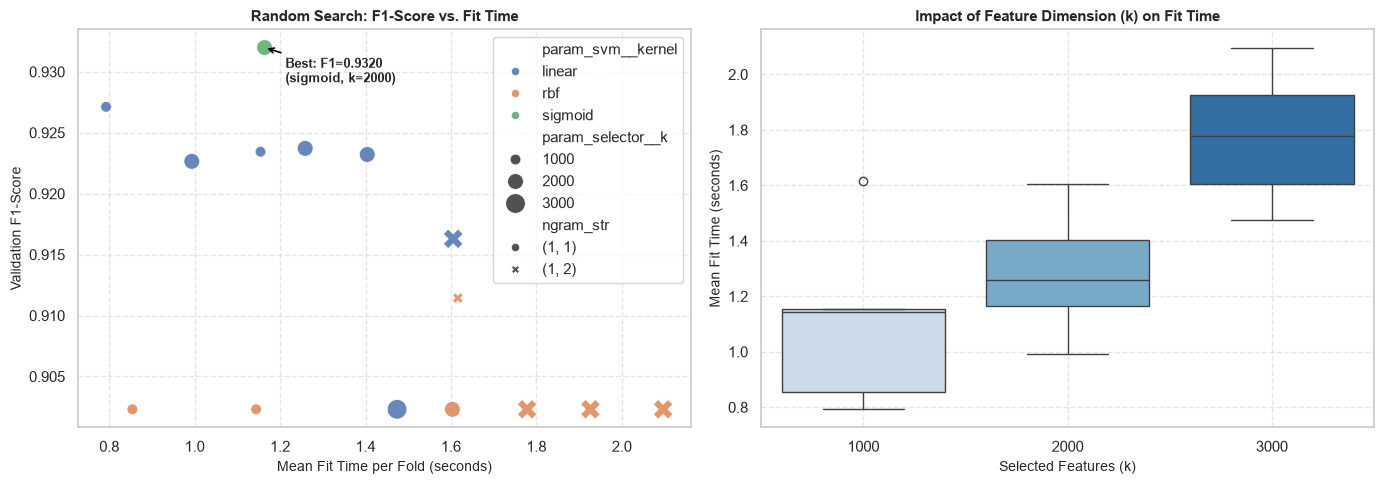
\includegraphics[width=0.88\textwidth]{figures/svm_cell20_0.png}
\caption{Phân bố F1-Score so với thời gian huấn luyện và ảnh hưởng của số đặc trưng $k$ trong quá trình tinh chỉnh SVM}
\label{fig:svm_tuning}
\end{figure}

\subsection{Kỹ thuật mở rộng nâng cao}

\subsubsection{Học kết hợp (Ensemble Learning)}
Nhằm cải thiện độ chính xác và giảm phương sai dự đoán cho mô hình SVM, hai kỹ thuật học kết hợp được thử nghiệm trên không gian vector đặc trưng TF-IDF:
\begin{itemize}
    \item \textbf{Bagging}: Giảm phương sai bằng cách huấn luyện song song nhiều mô hình cơ sở (\texttt{LinearSVC}) trên các tập con mẫu lấy ngẫu nhiên có hoàn lại (\textit{Bootstrap Aggregating}, \texttt{n\_estimators=10}, \texttt{max\_samples=0.8}).
    \item \textbf{AdaBoost}: Giảm độ chệch bằng cách huấn luyện tuần tự các bộ phân loại yếu, tập trung tăng trọng số cho các mẫu bị phân loại sai ở bước trước (\textit{Adaptive Boosting}, \texttt{n\_estimators=50}).
\end{itemize}

\begin{table}[H]
\centering
\begin{tabular}{|l|c|c|}
\hline
\textbf{Mô hình Ensemble} & \textbf{Accuracy} & \textbf{F1-Score} \\ \hline
Bagging & \textbf{0.8934} & \textbf{0.9369} \\ \hline
AdaBoostClassifier & 0.8412 & 0.9113 \\ \hline
\end{tabular}
\caption{So sánh hiệu năng giữa hai phương pháp Ensemble Learning}
\label{tab:ensemble_eval}
\end{table}

\begin{figure}[H]
\centering
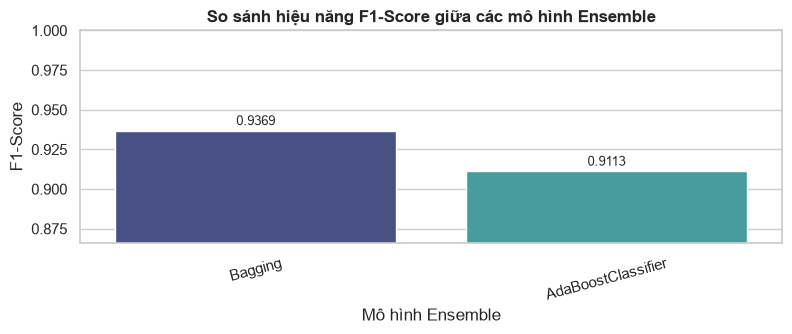
\includegraphics[width=0.62\textwidth]{figures/svm_cell24_0.png}
\caption{So sánh hiệu năng F1-Score giữa các phương pháp Ensemble}
\label{fig:ensemble_chart}
\end{figure}

Kết quả ở Bảng~\ref{tab:ensemble_eval} và Hình~\ref{fig:ensemble_chart} cho thấy Bagging đạt hiệu năng vượt trội rõ rệt so với AdaBoost trên không gian đặc trưng văn bản nhiều chiều. Do đó, kiến trúc Bagging được tích hợp vào mô hình SVM cuối cùng.

\subsubsection{Tích hợp siêu dữ liệu (XGBoost with Metadata)}
Bên cạnh văn bản đánh giá thuần túy, bộ dữ liệu còn cung cấp các thông tin ngữ cảnh gồm độ tuổi khách hàng (\texttt{Age}) và danh mục sản phẩm (\texttt{Division Name}, \texttt{Department Name}, \texttt{Class Name}). Kiến trúc \texttt{ColumnTransformer} được xây dựng để ghép nối:
\begin{itemize}
    \item Đặc trưng văn bản: \texttt{TfidfVectorizer} với các siêu tham số tối ưu tìm được từ XGBoost.
    \item Đặc trưng phân loại danh mục: Mã hóa One-Hot (\texttt{OneHotEncoder(handle\_unknown='ignore')}).
    \item Đặc trưng số học: Cột \texttt{Age} truyền trực tiếp (\texttt{passthrough}).
\end{itemize}
Mô hình kết hợp \texttt{XGBoost + metadata} được huấn luyện và đánh giá trên tập kiểm thử nhằm kiểm chứng mức độ đóng góp của dữ liệu dạng bảng bổ trợ vào quyết định phân loại.

\subsubsection{Xây dựng Pipeline hoàn chỉnh cho mô hình SVM}
Tổng hợp các kết quả thực nghiệm về trích xuất đặc trưng, lựa chọn đặc trưng, siêu tham số và học kết hợp, mô hình SVM cuối cùng được xây dựng thành một quy trình khép kín:
\begin{enumerate}
    \item \textbf{Vector hóa}: Sử dụng \texttt{TfidfVectorizer} với các siêu tham số: \texttt{max\_features} = 5000, \texttt{ngram\_range} = (1, 1) và \texttt{sublinear\_tf} = False.
    \item \textbf{Lọc đặc trưng}: \texttt{SelectKBest} ($\chi^2$, $k = 2000$), giảm số chiều đặc trưng từ $(18788, 5000)$ xuống $(18788, 2000)$.
    \item \textbf{Học tổ hợp}: \texttt{BaggingClassifier} sử dụng bộ phân loại cơ sở \texttt{SVC} (kernel Sigmoid, $C = 0.5$, $\gamma = \text{scale}$), \texttt{n\_estimators} = 10, tỷ lệ lấy mẫu con \texttt{max\_samples} = 0.8.
\end{enumerate}
Mô hình hội tụ trong 17.57 giây và hoàn tất toàn bộ quá trình xử lý - đánh giá trong 25.17 giây, đạt độ chính xác kiểm thử 90\% và Macro-F1 là 0.80.
